\section{Introducción}
\begin{frame}{Introducción}
	\begin{block}{Chat}
		En esta práctica crearemos un chat multiusuario usando el paradigma cliente-servidor. El servidor será
		un proceso alojado en alguno de los ordenadores de la comunicación. 
		
		Usaremos como host la dirección IP local.
	\end{block}
	\begin{alertblock}{Cuidado}
		Hay redes wifi que bloquean los ping que se mandan, por eso
		hay que tener especial cuidado a la hora de ejecutar los programas.
	\end{alertblock}
\end{frame}


% -----------------------------------


\begin{frame}{Introducción}
	\begin{block}{Esquema}
		El esquema que usaremos será una clase \textit{Writer} y una clase \textit{Printer}, la primera se encargará de mandar los mensajes al servidor, la segunda de recibirlos y mostrarlos con el formato adecuado.
	\end{block}
\end{frame}


% -----------------------------------


\begin{frame}{Introducción}
	\begin{exampleblock}{Esquema}
		\begin{figure}[H]
    		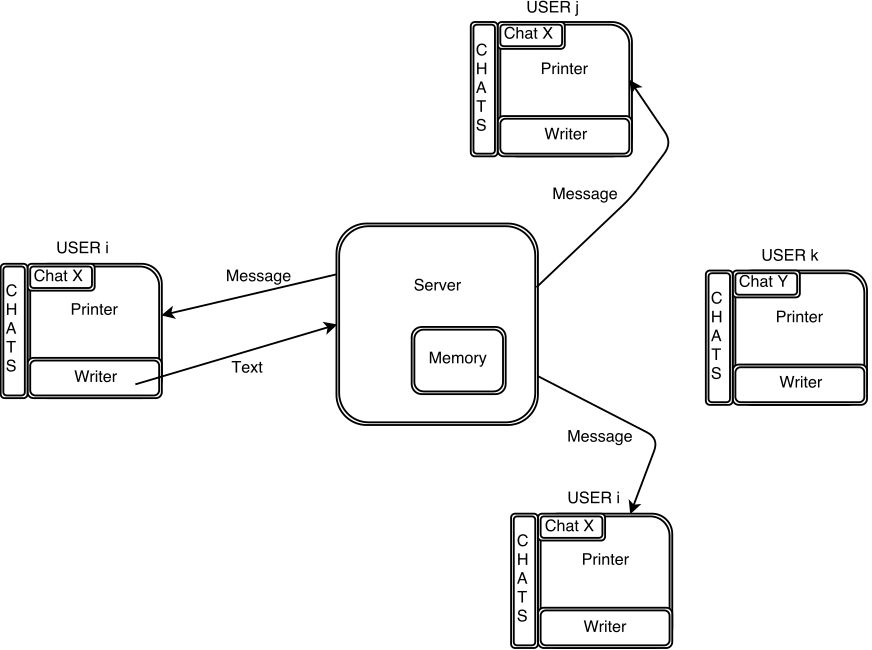
\includegraphics[scale=0.31]{./Imagenes/chat.png}
		\end{figure}
	\end{exampleblock}
\end{frame}